\documentclass[UTF8]{ctexart}
\usepackage{graphicx}
\usepackage{listings}

\title{实验四报告}
\author{唐灵\\519030910052\\F1903002}
\date{\today}
\begin{document}
    \maketitle
    \begin{abstract}
        这是电工导c课程的第三次实验
    \end{abstract}
    \section{实验概览}
        本次实验是对于爬虫与文本检索的一个综合简单应用,重点在于应用lucene建立索引并进行简单的搜索。
    \section{实验环境}
    本次实验的所有代码在电类工程导论c课程中在课程方统一给定的“ee208”$Docker$容器中运行并实现。
    \section{练习解决思路}
        \subsection{爬虫的解决思路}
            爬虫的的话,直接采用lab2中的代码,需要注意的是关于网页编码的问题,一定要查看过后进行修改再进行爬取。
            由于我采用的是在建立索引的时候进行文档处理,所以这一步直接保留网页的源代码和文件名与网页链接的对应关系即可。
        \subsection{建立索引的解决思路}
            建立索引,需要建立五个字段,分别是文件名,本地路径,网页链接,文档标题,以及文档内容,我们只需要对于最后一个字段进行分析即可,
            因为前面的几个字段实际上是不可读的,添加倒排索引也并没有什么意义。\par
            从爬取下来的页面中,分别对于五个字段进行读取:
            \begin{enumerate}
                \item 文件名(name):直接读取
                \item 本地路径(path):将文件夹路径以及文件名组合形成本地路径
                \item 网页链接(url):将index.txt文件路径作为一个建立索引类的初始化参量,读取index.txt文件,形成一个文件名到网页链接的字典,通过文件名,得到网页链接。
                \item 文档标题(title):读取网页源文件,利用BeautifulSoup库找到<title>标签,读取其中的字符串作为文档标题。
                \item 文档内容(contents):利用BeautifulSoup库,去除文档中的所有标签,再利用jieba的lcut方法进行中文分词,再利用join方法并将间隔内容变为空格,
                自然的,我们的分词器应当使用WhitespaceAnalyzer,利用空格分词,建立索引。
            \end{enumerate}
            这样我们建立索引的工作就基本上完成了。
        \subsection{搜索结果解决思路}
            对于搜索,我们对于代码的修改主要集中在两个方面:
            \begin{enumerate}
                \item 第一是要将url等更多的信息给打印出来,这个是很好办的,只需要改变一下读取文档的字段以及打印的格式即可。
                \item 第二个问题主要集中在如何对于中文语段达到比较好的搜索效果,如果输入的词较为短的话当然可以得到比较好的效果,直接搞进去就行。\par
                但是如果输入的是一句话,基本上不可能完全匹配(内容和顺序),所以考虑在进入搜索之前对于语句进行适当的处理,使得其成为一个布尔语句,用AND连接,这样至少突破了顺序完全匹配的限定,可以得到不错的效果。\par
                实现也是不难的,使用jieba分词,并将间隔词设定为" AND ",使用join方法即可获得一个布尔语句。
            \end{enumerate}
    \section{代码运行结果}
        \subsection{爬虫的运行结果}
            \begin{figure}[ht]
                \centering
                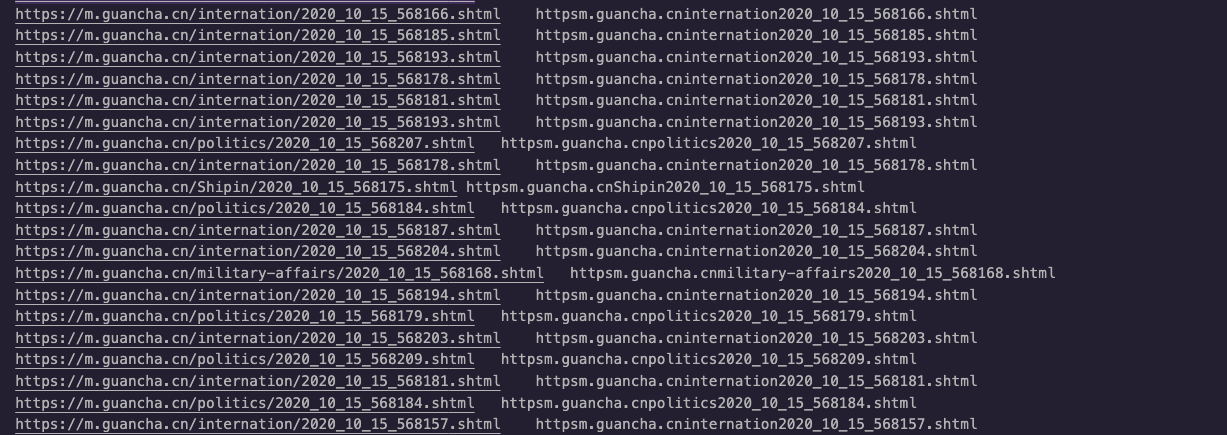
\includegraphics[scale=0.25]{img/index.png}
                \caption{index.txt文件内容(存储文件名与网页链接的关系)}
            \end{figure} 
            \begin{figure}[ht]
                \centering
                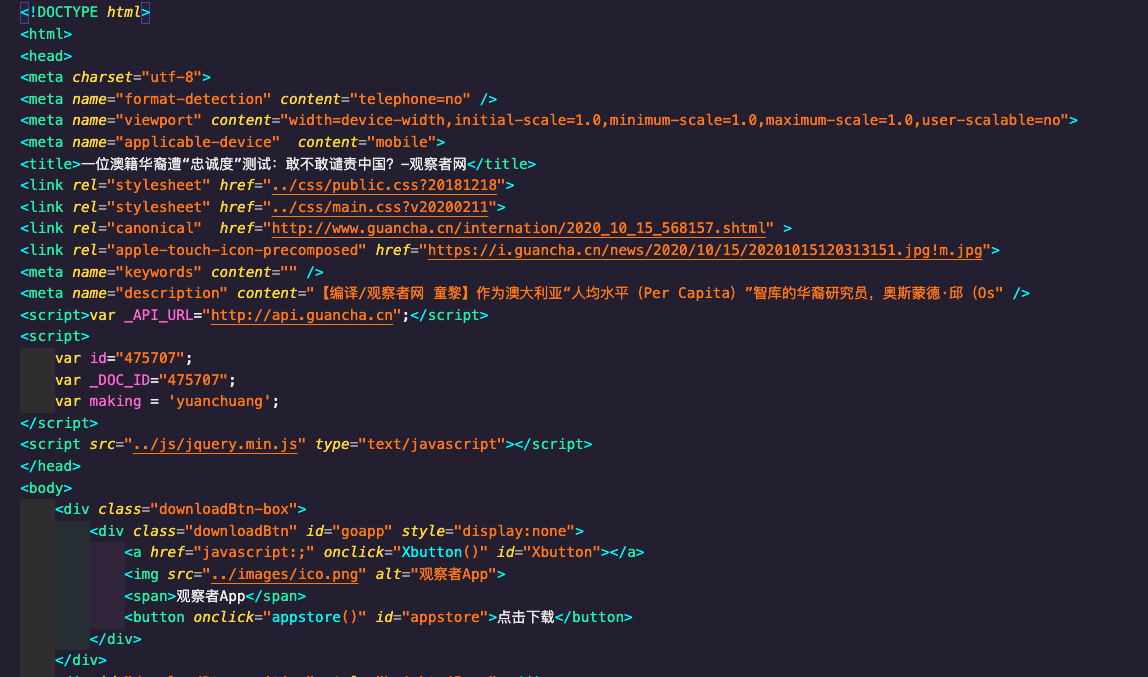
\includegraphics[scale=0.25]{img/shtml.png}
                \caption{存下来的网页源代码(部分)}
            \end{figure}
        \subsection{建立索引的运行结果}
            \begin{figure}[ht]
                \centering
                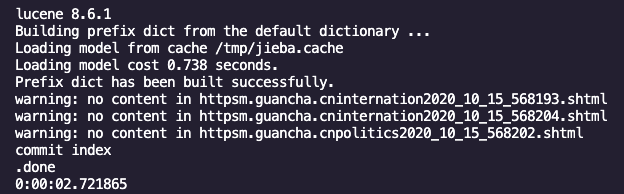
\includegraphics[scale=0.5]{img/create_index.png}
                \caption{建立索引过程中终端打印信息}
            \end{figure}
        \subsection{搜索结果的运行结果}
            \begin{figure}[ht]
                \centering
                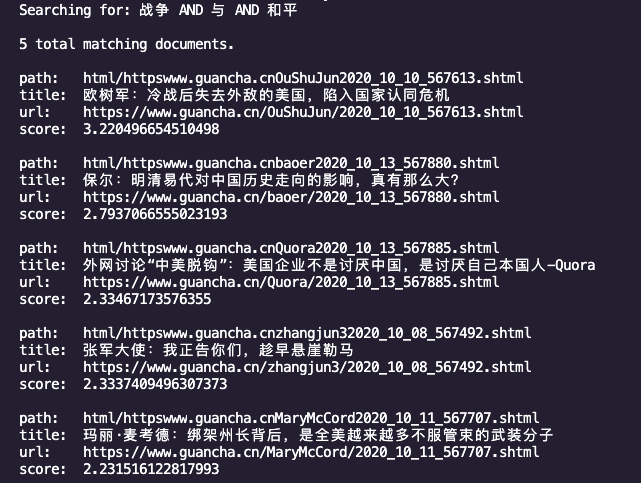
\includegraphics[scale=0.5]{img/search_result.png}
                \caption{搜索内容为“战争与和平”的搜索结果}
            \end{figure}

\end{document}